\chapter{Cómo se hacen mayores los animales}\label{ch:g2:animals-grow-up}

Un gatito parece un gato pequeño desde su primer día. Pero la rana de
la charca empezó siendo un renacuajo con forma de pez y sin patas, y
la mariposa de la budleya pasó semanas siendo una \omterm{ex:g2:animals-grow-up:butterfly}{oruga} que se
arrastraba. No todas las crías se parecen a sus padres --- algunas
tienen que transformarse por completo camino de la edad adulta.

\section{Del huevo o nacidos vivos}

\begin{definition}[Dos maneras de nacer]\label{def:g2:animals-grow-up:born}
Las crías de los \omterm{def:g1:animals-around-us:animal}{animales} llegan al mundo de dos maneras:
\begin{itemize}
  \item casi todas salen de un \emph{huevo}\index{huevo} puesto por la
        madre: aves, peces, ranas, caracoles, insectos;
  \item otras \emph{nacen vivas}\index{nacer vivo}, salen ya formadas
        del cuerpo de la madre y beben su \emph{leche}\index{leche}:
        gatos, perros, vacas, conejos --- y las personas.
\end{itemize}
\end{definition}

\begin{example}[En el gallinero y en la cesta]\label{ex:g2:animals-grow-up:henhouse}
La gallina pone \omterm{def:g2:animals-grow-up:born}{huevos} y se echa sobre ellos para mantenerlos
calientes; tres semanas después, los pollitos rompen la cáscara y
salen. En la cesta de al lado de la estufa, los gatitos de la gata
nacieron vivos esa misma noche y encontraron su \omterm{def:g2:animals-grow-up:born}{leche} en menos de una hora.
\end{example}

\begin{remark}[Un huevo no es una piedra]\label{rem:g2:animals-grow-up:egg}
Dentro de un \omterm{def:g2:animals-grow-up:born}{huevo} incubado se está construyendo un pollito en
silencio, alimentado por la yema amarilla. El \omterm{def:g2:animals-grow-up:born}{huevo} no espera --- está
trabajando. Por eso la gallina mantiene calientes sus \omterm{def:g2:animals-grow-up:born}{huevos}, y por
eso no hay que echarle la culpa al frío de un \omterm{def:g2:animals-grow-up:born}{huevo} de la nevera, que
nunca iba a dar un pollito.
\end{remark}

\section{Crecer sin transformarse}

\begin{definition}[Crecer igual que los padres]\label{def:g2:animals-grow-up:direct}
Muchas crías son \emph{miniaturas de sus
padres}\index{miniatura de los padres}: el gatito es un gato pequeño,
el potro un caballo pequeño, el pollito una gallina pequeña. Para
ellos, hacerse mayores es hacerse más grandes y más fuertes --- la
forma del cuerpo no cambia.
\end{definition}

\begin{example}[Del gatito al gato]\label{ex:g2:animals-grow-up:kitten}
El gatito recién nacido bebe \omterm{def:g2:animals-grow-up:born}{leche} con los \omterm{def:g1:the-five-senses:sense}{ojos} cerrados. Al mes juega
y da zarpazos; a los seis meses caza como un gato adulto; al año es
adulto, quizá con gatitos propios. Gato pequeño, gato más grande,
gato: la misma forma durante todo el camino.
\end{example}

\section{Crecer transformándose}

\begin{definition}[Metamorfosis]\label{def:g2:animals-grow-up:metamorphosis}
Algunas crías no se parecen en nada a sus padres y tienen que cambiar
la forma entera de su cuerpo para convertirse en adultas. Ese gran
cambio se llama \emph{metamorfosis}\index{metamorfosis}. El renacuajo
se convierte en rana; la \omterm{ex:g2:animals-grow-up:butterfly}{oruga} se convierte en mariposa.
\end{definition}

\begin{example}[El camino de la rana]\label{ex:g2:animals-grow-up:frog}
De los \omterm{def:g2:animals-grow-up:born}{huevos} de rana de la charca salen \emph{renacuajos}\index{renacuajo}:
cabeza redonda, cola larga, sin patas, que respiran en el agua como
los peces. Después, semana a semana: aparecen las patas traseras y
luego las delanteras; la cola se encoge hasta desaparecer; y un día
una ranita sale a la orilla. El mismo \omterm{def:g1:animals-around-us:animal}{animal} --- reconstruido.
\end{example}

\begin{omfigure}
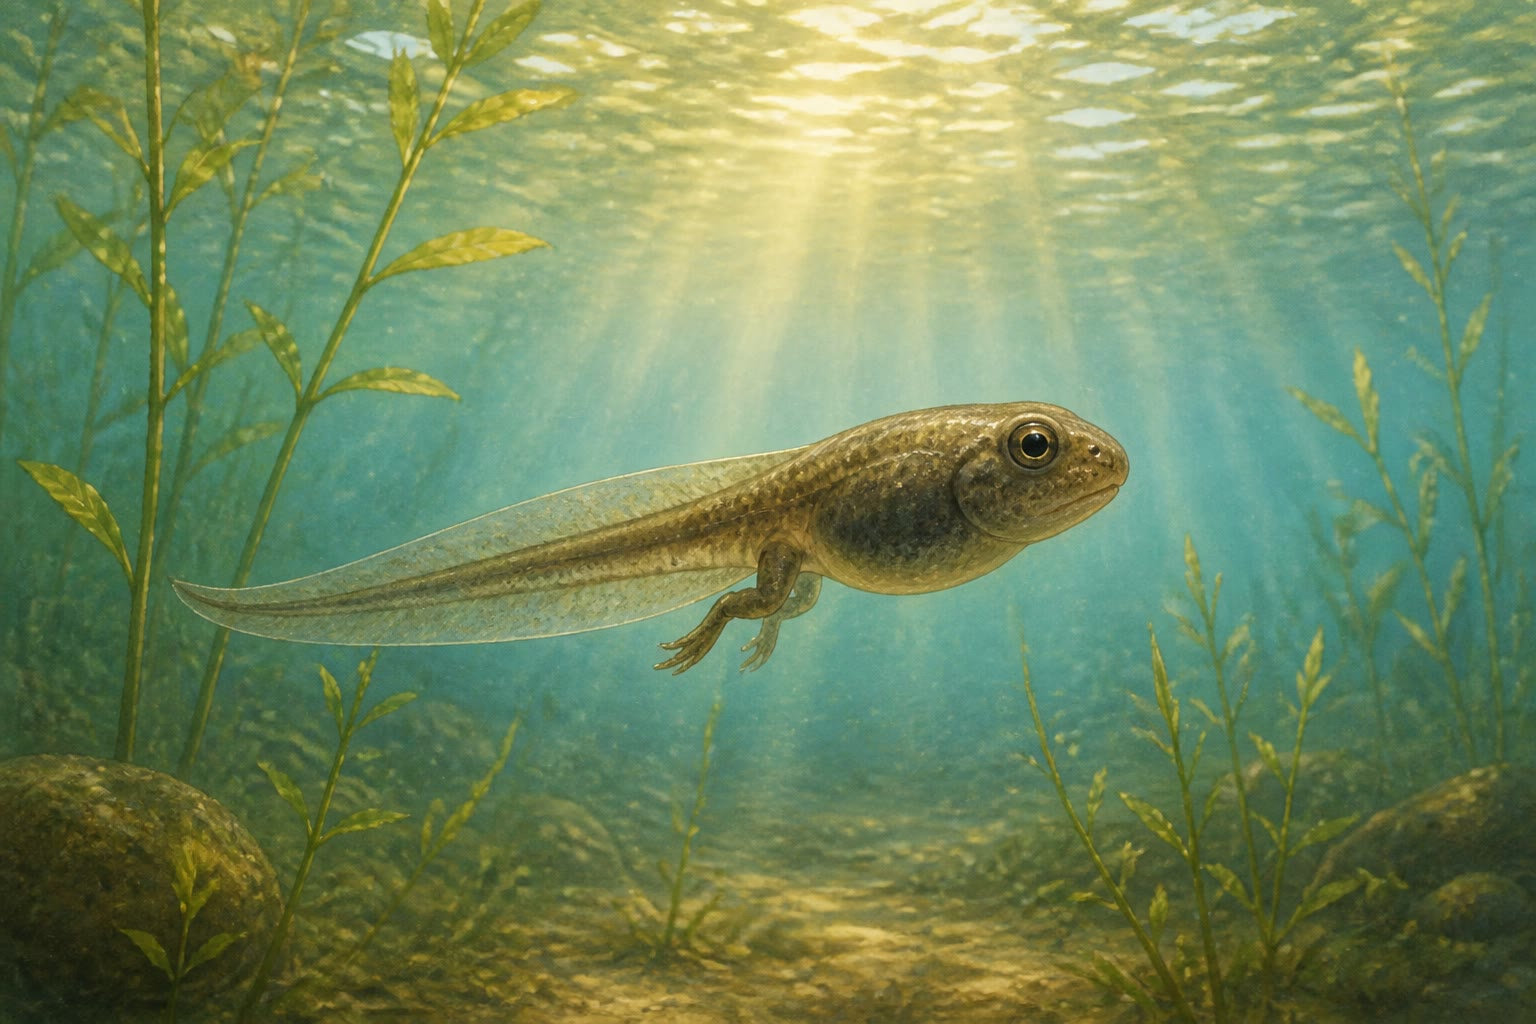
\includegraphics[width=0.6\linewidth]{images/book1/ai/g2-grow-tadpole.jpg}

{\small Sorprendida en plena \omterm{def:g2:animals-grow-up:metamorphosis}{metamorfosis}: patas traseras ya crecidas,
patas delanteras aún por salir, cola todavía larga.}
\end{omfigure}

\begin{omfigure}
\begin{tikzpicture}
  \node[anchor=south west, inner sep=0] (img) at (0,0)
    {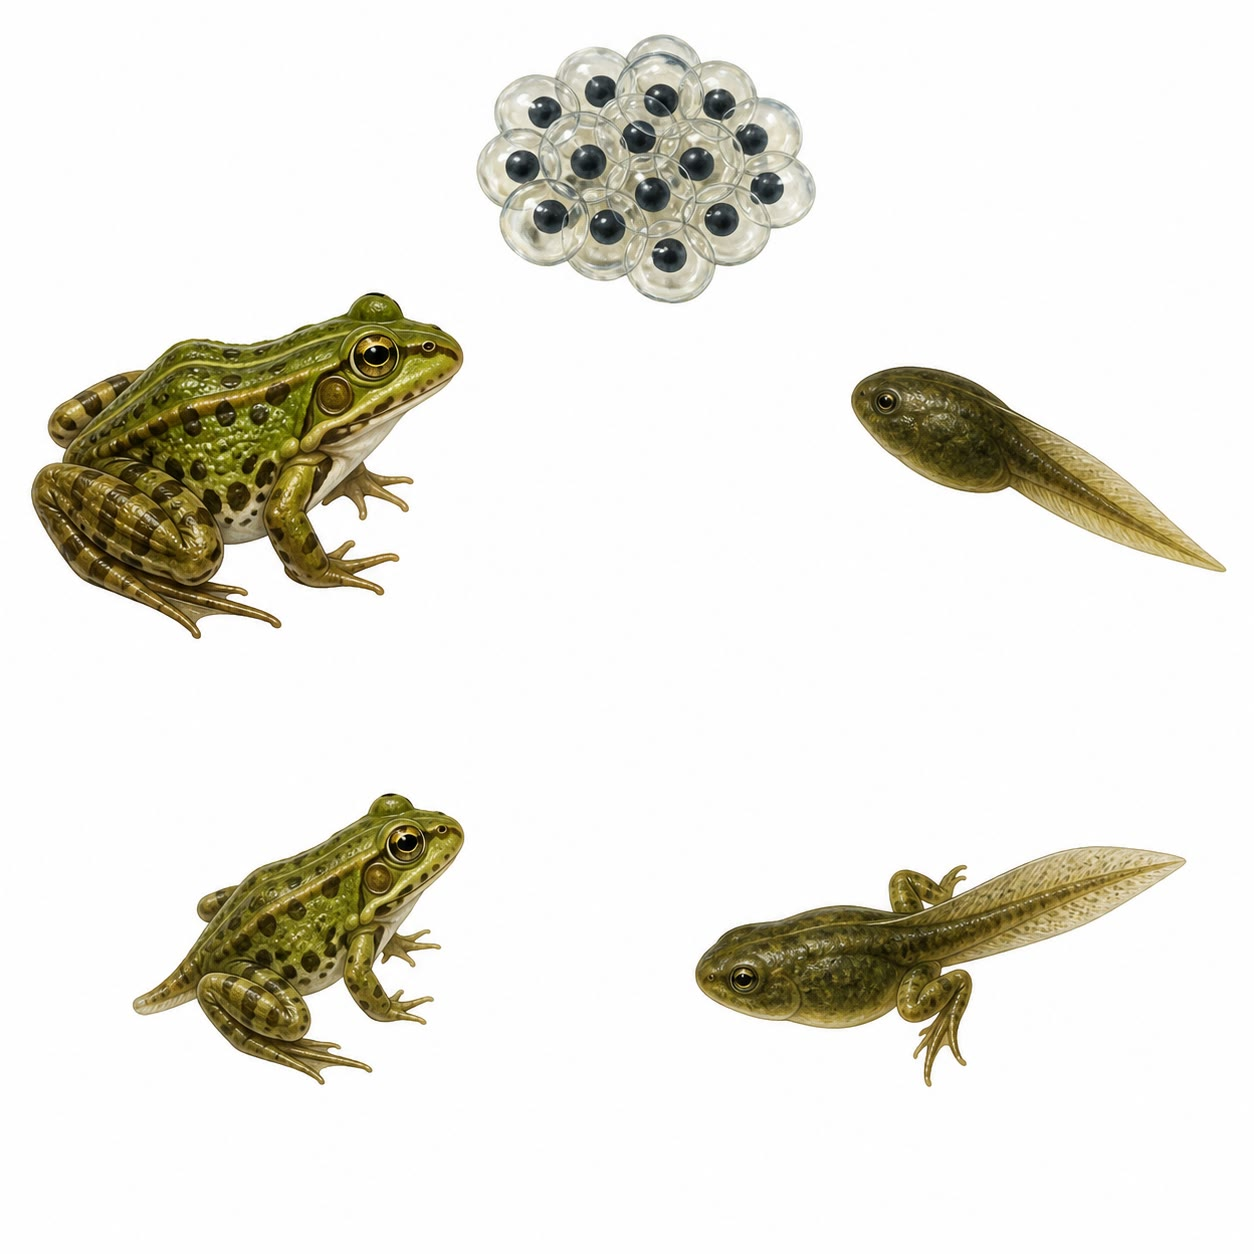
\includegraphics[width=0.72\linewidth]{images/book1/ai/fig-frog-cycle.jpg}};
  \begin{scope}[x={(img.south east)}, y={(img.north west)},
      every node/.style={font=\small}]
    \node[above] at (0.33,0.92) {huevos en la charca};
    \node[right, align=left] at (0.87,0.44)
      {renacuajo:\\ cola, sin patas};
    \node[below, align=center] at (0.80,0.05)
      {salen las patas traseras\\ y luego las delanteras};
    \node[below] at (0.22,0.05) {la cola se encoge: una ranita};
    \node[left, align=right] at (0.075,0.78) {rana adulta};
    \draw[->, thick, omProp] (0.70,0.86) to[bend left=20] (0.87,0.68);
    \draw[->, thick, omProp] (0.88,0.38) to[bend left=15] (0.85,0.25);
    \draw[->, thick, omProp] (0.60,0.16) to[bend left=12] (0.42,0.14);
    \draw[->, thick, omProp] (0.16,0.32) to[bend left=15] (0.13,0.48);
    \draw[->, thick, omProp] (0.30,0.80) to[bend left=18] (0.42,0.88);
  \end{scope}
\end{tikzpicture}

{\small La \omterm{def:g2:animals-grow-up:metamorphosis}{metamorfosis} de la rana, girando en el sentido de las
agujas del reloj desde los \omterm{def:g2:animals-grow-up:born}{huevos}: renacuajo, patas, ranita, adulta
--- y la adulta pone los \omterm{def:g2:animals-grow-up:born}{huevos} siguientes.}
\end{omfigure}

\begin{example}[El camino de la mariposa]\label{ex:g2:animals-grow-up:butterfly}
Del \omterm{def:g2:animals-grow-up:born}{huevo} de la mariposa sale una \emph{oruga}\index{oruga}, que casi
solo come \omterm{def:g1:plants-around-us:parts}{hojas} y crece. Un día se envuelve en un estuche, la
\emph{crisálida}\index{crisálida}, y deja de moverse. Dentro, el
cuerpo se reconstruye; al cabo de unas semanas el estuche se abre y
sale una mariposa, que despliega sus alas nuevas y húmedas. \omterm{def:g2:animals-grow-up:born}{Huevo},
\omterm{ex:g2:animals-grow-up:butterfly}{oruga}, \omterm{ex:g2:animals-grow-up:butterfly}{crisálida}, mariposa: cuatro etapas de un mismo \omterm{def:g1:animals-around-us:animal}{animal}.
\end{example}

\begin{method}[Leer el ciclo de vida de un animal]\label{met:g2:animals-grow-up:read}
Para cualquier \omterm{def:g1:animals-around-us:animal}{animal} que te encuentres:
\begin{enumerate}
  \item pregunta cómo nace: ¿de un \omterm{def:g2:animals-grow-up:born}{huevo} o vivo?
  \item pregunta a qué se parece la cría: ¿a una miniatura de sus
        padres o a otra cosa?
  \item si tiene otra forma, se transformará: busca las etapas de su
        \omterm{def:g2:animals-grow-up:metamorphosis}{metamorfosis};
  \item dibuja el ciclo como una rueda, con una flecha que vuelva del
        adulto a los \omterm{def:g2:animals-grow-up:born}{huevos}.
\end{enumerate}
\end{method}

\begin{remark}[Leche, o al trabajo desde el primer día]\label{rem:g2:animals-grow-up:care}
A los gatitos su madre los alimenta y los lava durante semanas; un
renacuajo recién salido no recibe ninguna ayuda y tiene que
alimentarse solo desde el primer día. A unas crías las cuidan, otras
empiezan la vida solas --- los dos caminos llevan a la edad adulta.
\end{remark}

\section{Ejercicios}

\begin{exercise}[$\star$]\label{exo:g2:animals-grow-up:1}
Di las dos maneras en que las crías llegan al mundo, con un ejemplo de
cada una.
\end{exercise}

\begin{exercise}[$\star$]\label{exo:g2:animals-grow-up:2}
¿De un \omterm{def:g2:animals-grow-up:born}{huevo} o nacido vivo: (a) un pollito? (b) un gatito? (c) una
rana? (d) un conejo? (e) un caracol?
\end{exercise}

\begin{exercise}[$\star$]\label{exo:g2:animals-grow-up:3}
¿Qué bebe primero un gatito? ¿Qué \omterm{def:g1:animals-around-us:animal}{animales} de este capítulo beben lo
mismo al nacer?
\end{exercise}

\begin{exercise}[$\star$]\label{exo:g2:animals-grow-up:4}
¿Qué es la \omterm{def:g2:animals-grow-up:metamorphosis}{metamorfosis}? Nombra los dos ejemplos famosos de este
capítulo.
\end{exercise}

\begin{exercise}[$\star$]\label{exo:g2:animals-grow-up:5}
Ordena las etapas de la rana: rana --- \omterm{def:g2:animals-grow-up:born}{huevos} --- renacuajo con patas
--- renacuajo.
\end{exercise}

\begin{exercise}[$\star$]\label{exo:g2:animals-grow-up:6}
Ordena las etapas de la mariposa: mariposa --- \omterm{ex:g2:animals-grow-up:butterfly}{oruga} --- \omterm{def:g2:animals-grow-up:born}{huevo} ---
\omterm{ex:g2:animals-grow-up:butterfly}{crisálida}. ¿En qué etapa come \omterm{def:g1:plants-around-us:parts}{hojas} el \omterm{def:g1:animals-around-us:animal}{animal} y es cuando más crece?
\end{exercise}

\begin{exercise}[$\star$]\label{exo:g2:animals-grow-up:7}
¿Qué cría es una miniatura de sus padres: el renacuajo o el potro?
¿Qué significa hacerse mayor para esa?
\end{exercise}

\begin{exercise}[$\star$]\label{exo:g2:animals-grow-up:8}
¿Por qué se echa la gallina sobre sus \omterm{def:g2:animals-grow-up:born}{huevos}? ¿Qué está pasando dentro
de ellos, según la \cref{rem:g2:animals-grow-up:egg}?
\end{exercise}

\begin{exercise}[$\star\star$]\label{exo:g2:animals-grow-up:9}
En la charca, Zoe encuentra un \omterm{def:g1:animals-around-us:animal}{animal} pequeño con la cabeza redonda,
la cola larga, dos patas traseras y sin patas delanteras. Con la
figura del ciclo de la rana, di exactamente dónde está en su camino,
qué era antes y qué viene después.
\end{exercise}

\begin{exercise}[$\star\star$]\label{exo:g2:animals-grow-up:10}
``La \omterm{ex:g2:animals-grow-up:butterfly}{oruga} murió dentro del estuche y una mariposa se mudó allí''.
¿Qué pasó de verdad dentro de la \omterm{ex:g2:animals-grow-up:butterfly}{crisálida}? Responde con la
\cref{def:g2:animals-grow-up:metamorphosis} y el
\cref{ex:g2:animals-grow-up:butterfly}.
\end{exercise}
